\chapter{Introduction} \label{ChapIntroduction}
GIRAF is a series of applications(apps) for Android, intended to help citizens with autism in their everyday life. Over the past four years GIRAF have been developed by students at Aalborg University, with a new group of students taking the mantle every year. As a result of this, it was hard to get an overview of the project in its entirety. We here give an overview of the GIRAF project as it was, when we started working on it, and we also give some insight into the organization of the project.

\section{Status of GIRAF} %To add: pictures to help descripe apps.
At the start of the project all the apps were on Google Play, and most of the apps were executable, except for two of the apps which crashed instantly. Most of the executable apps also had some bugs which in some of the apps could lead to a crash. All of the apps on Google Play were release-versions, but since some of them could not even be executed, it might have been better to have those on the store as alpha or beta-versions.

\section{Multiproject, Subprojects, and Responsibility} %To add better description of Scrum of Scrums principle.
The overall goal for the multiproject this year was, to make a working system that is usable and stable. A multiproject in this context being an overall project that several groups, in this case all 6th semester software groups, work on in collaboration. In order to achieve a better workflow, the project was split into three subprojects: Database (DB), Graphical User Interface(GUI), and Build and Deployment(B\&D). Our group were a part of B\&D, along with 3 other groups. Both the DB and GUI subprojects had 5 groups each. See Figure \ref{ScrumOfScrumsOverview} for an overview of the structure of this years multiproject.

\begin{figure}
	\centering
	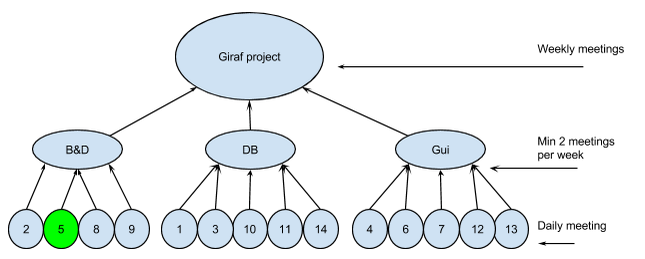
\includegraphics[width=0.8 \textwidth]{pictures/ScrumOfScrum.png}
	\caption{Overview of the project structure with sub-projects and the individual groups depicted, our group is marked with green.}
	\label{ScrumOfScrumsOverview}
\end{figure}

\subsection{Database}
DB groups were responsible for handling all things database related, this included making current data accessible and adding new data to the database, as per request from other groups or as needed.

\subsection{Graphical User Interface}
GUI groups were mainly responsible for developing the different apps, this included making general changes in the apps and bug fixing anything related to the apps.

\subsection{Build and Deployment}
B\&D groups were responsible for most of the internal project matters, this included maintaining the server services, developing and maintaining the automatic build tools, handling publication of the apps, and administrating the version control.

\section{Project organization}
The project is organized using Scrum principles where the individual subprojects held Scrum of Scrum meetings twice a week. The individual groups can follow any principles that they would like, but Scrum was recommended. Our group decided to follow Scrum to have the same structure as the project.
In addition an overall meeting was held every week where at least one representative from each group were present. At these meetings the overall status for each subproject were given, and any decisions that needed overall consensus were discussed.

As the overall structure is Scrum, the project was split into four sprints. The first sprint was devoted to bug fixing, user stories and tasks that were still unsolved from last year, and setting up and organizing project tools. In regards to user stories, it was decided early on at an overall meeting, to operate with two types of user stories, those from the costumers, these were called user stories; and those from the other groups, called developer stories. For consistencies sake we will just refer to both as user stories in the report, as the difference was mainly a concern when groups from different subprojects where discussing internally.

\subsection{Roles and responsibilities}
To get a better start and to delegate some responsibilities out, some groups were given roles, so that the groups knew, which groups were responsible for what, and so that people knew where to go, if there was anything in the project they had trouble with.


\textbf{Process:}
Responsible for assuring that the overall project follows the scrum principles, and for informing other group about the process used in the project.

\textbf{Configuration Management:}
Responsible for keeping track of the different versions of the apps, and for making sure that only working version of the apps are released.

\textbf{Google Play:}
Responsible for managing the apps on the Google Play store, and for having the apps uphold the rules for having them on the store. This was one of our responsibilities.

\textbf{Google Analytics:}
Responsible for sending crash report from Google Analytics, to the groups that request the information, and for making a guide for how to implement the Google Analytics API in the apps. This was also one of our responsibilities.

\textbf{Product Owner:}
This role was given to three groups, one for each sub-project. The product owners are responsible for keeping track of the user stories that are assigned to their sub-project, and for organizing the sprint planning and sprint end. We were responsible for the B\&D sub-project as product owners.

\textbf{Issue Tracker:}
Responsible for setting up a system on redmine for keeping track of user stories and for informing group if they do not finish a user story in tie or forget to change the status of the user story on redmine. The group responsible for this did set up a system for user stories, but as time progressed, groups stopped using the system and in the end this role was more or less removed.

\textbf{Server:}
Responsible for the server the project uses, this includes installing software on the server, upgrading the capacity of the server, and making sure the server is running.

\textbf{Redmine in General:}
Responsible for keeping track of whether the redmine website was running and for fixing the site if any problem should occur.

\textbf{Redmine Wiki:}
Responsible for keeping the redmine wiki running and for being the goto group if anyone have problem setting up a wiki page on redmine.

\textbf{Redmine Forum:}
Responsible for keeping the redmine forum running.
 
\textbf{Git:}
Responsible the git system used in our project, and for making changes to it if requested. For this role they made a guide

\textbf{Webadmin:}
Responsible for keeping the Giraf website running (insert link) and for updating information on the site when needed.

\textbf{Android Guru}
This role was given to a person that at the start of the project already had a lot of experience with android, and worked as a goto guy, if anyone had any troubles that were android related.

\textbf{Graphics Guidelines:}
This group was responsible for finding graphical guidelines that should be used for the apps, so that all apps had a consistent look.

\textbf{Code Style:}
This group was responsible for finding guidelines for how code should be written and for writing a guide so that all groups had a common place to find these guidelines.


\textbf{Customer Representatives:}
This group was responsible for managing the contact between the project and the customers, so that not all group send them emails all the time and so that if multiple groups have the same question, the question is only asked once.


\section{Tools used in the project}
In this section we describe some of the tools used in the project.

\subsection{Android Studio}
For coding the apps in the project, Android Studio was used, or more specifically Android Studio 1.1. It was an older version of Android Studio in the start, but already a few weeks into the project Android Studio was upgraded, to make use of the new features. Android Studio is an IDE made by Google, for coding apps for android devices \citep{AndroidStudio}

\subsection{Gradle}
To build the project in Android Studio Gradle was used, Gradle is a project automation tool, which is specially designed for use in multiprojects \citep{Gradle}. For our project we use it to build each app, and to make use of the maven repository we use for our libraries.

\subsection{Artifactory}
Artifactory is the maven repository that is used in the project to store and manage versions of libraries. Because it is able to store multiple versions of every library, it makes it possible to have apps that use an older version of a library and still be able to tell which version is used, and it is also easy to change the version of a library an app is using, by just changing an extension of a line of code in the Gradle build file of the app.

\subsection{Git}
Git is the tool that is used in the project for sharing files internally in the project, primarily code files for the apps. What makes Git good as a file sharing system is that it allows multiple people to code on the same program, and if you commit and another person had committed some changes before you, you can merge the changes between the two versions. Another functionality that Git has that is useful for this project is that it allows the use of “branches”, which allows people to code in a repository that is separate from the original (Master branch). This was used in the project to have one group work on one branch and then when the group wanted to get the changes tested on jenkins, they merged the branch with the master branch.

\subsection{Jenkins}
Jenkins is the tool used for building and testing all the apps before they are released. It is set up such that if anyone pushes changes to the master branch, the app on that branch is build and then tested by Jenkins. In addition to having tests run every time something is pushed on Git, Jenkins also makes an install test and “monkey test” for all apps every night. The install test try to install all apps on an emulator to test if any of the apps have a conflict when installed, and the monkey test, starts all the apps one by one and then pushes some random buttons to test if the app works when it is run on the emulator. When an app is built and tested successful the new version of the app is pushed to Google Play as an alpha-version.

\subsection{Google Play}
Google Play is the platform on which all the apps are published. By uploading the apps to Google Play the app become available on the Google Play store where everyone that has an android device can find and download them.

\subsection{Google Analytics}
Google Analytics was used in the project to get crash reports from the apps. When an app crashes a crash report is send to Google Analytics, where you can go and see them. In addition it is also possible to make Google Analytics send the crash report by mail.

\subsection{Redmine}
Redmine is a web-based project management and issue tracking tool \citep{Redmine}, and was used as such in the project. Redmine was in the project used to share user stories and for sharing information in general. This information was shared through a forum and a wiki page. The forum was mostly used to arrange social arrangements and other messages, were a little wait time was not a problem, and the wiki page was used for sharing guides, guideline, general information, and for summaries from project meetings.

\subsection{Google Docs}
Like the redmine wiki, Google docs was used for sharing information, but only for the project backlog and for summaries from meetings. The reason Google docs was used for these was that it allows multiple users to edit the same document simultaneously, so that it is not only one person that is forced to write summaries at the meetings, and for the backlog it allowed one screen to display what is being talked about while another can edit the content.